\documentclass[12pt, twoside, a4paper]{report}

\usepackage{amsmath}
\usepackage[toc, page]{appendix}
\usepackage{graphicx}
\usepackage[sort&compress]{natbib}
\usepackage{subcaption}
\usepackage[nottoc]{tocbibind}

% Location of the graphics files
\graphicspath{{figures/}}
% Set line spacing
\linespread{1.5}

\begin{document}

\title{Real-time Pedestrian Modelling: Implementing the Ensemble Kalman Filter
for an Agent-Based Model}
\author{Keiran Suchak --- 200888140}
\maketitle

\chapter*{\centering Abstract}
\addcontentsline{toc}{chapter}{Abstract}

This is the abstract.

\tableofcontents
\listoffigures
\listoftables

\chapter*{Notes}

\begin{itemize}
    \item What is data assimilation?
    \item What is the Ensemble Kalman Filter?
    \item What are Agent-Based Models?
    \item How do people model pedestrians?
    \item What happens when an agent in one of the ensemble member models tries
        to leave the station early? Because we're only doing state estimation
        (meaning just the agent coordinates), the agent won't get reactivated.
    \item Errors should converge on something relating to twice the exit
        distance.
    \item Signposting at the beginning of each chapter
    \item Don't need to review calibration too much
    \item Don't need to talk about different types of enkf's too much
    \item Don't need to talk about DA with CA too much
\end{itemize}

%\section*{Structure}

%\begin{itemize}
    %\item What is the problem?
    %\item Why should people care?
    %\item What has been done in the past to try to solve the problem?
    %\item What are we doing to solve the problem? How is this different?
    %\item How well does our attempt work? How does this compare to others?
%\end{itemize}

\chapter{Introduction}\label{ch:intro}

A better understanding of how people move around their environment is of great
utility to both academics and policy-makers.
Such knowledge can be made use of in the contexts of urban planning, event
management and emergency response, particularly when considering urban
environments.
Furthermore, this may also be of use to those interested in the social issues of
mobility, inclusivity and accessibility of opportunities.

When considering such concepts, investigators often make use of modelling
techniques.
At their most fundamental, models represent our understanding of
the system that we are studying --- an understanding that may not be perfect
\citep{stanislaw1986tests}.
There exist modelling techniques for the simulation of how pedestrians move
around urban spaces.
However, these methods exist largely in isolation of the real-world --- that is
to say that whilst the simulations aim to reflect the real-world, there is no
method by which we can incorporate up-to-date observations into these models to
stop their divergence from reality.

Simulating pedestrian behaviour is often undertaken at the micro-scale, with
such models typically aiming to model at the individual level or on a spatially
fine-grained grid \citep{burstedde2001simulation}.
One of the most prevalent simulation methods in this field is that of
Agent-Based Modelling.
Such methods consist of two key components: agents and environments.
In an Agent-Based Model, we prescribe sets of rules by which individuals interact with each
other and their local environments; as interactions take place on the
micro-scale, we typically observe the emergence of structure at the macro-scale
such as crowding \citep{batty2003discrete} or lane formation \citep{liu2014agent}.
The evaluation of these rules is often not deterministic and instead
introduces some element of randomness; these stochastic elements aim to emulate
the variability of human behaviour.
The introduction of such randomness in conjunction with an imperfect
understanding of the phenomena at play, however, typically result in simulation
runs diverging from the real system.

In constructing their models, agent-based modellers undertake a development
process that involves model verification, validation and calibration.
We can take these to mean the following:
\begin{itemize}
    \item \textbf{Model verification}: the process of ensuring that the implementation is
        an accurate representation of the model \citep{xiang2005verification}.
    \item \textbf{Model validation}: the process of ensuring that the chosen model is an
        accurate representation of the phenomenon that we wish to study
        \citep{crooks2008key}.
    \item \textbf{Model calibration}: the process of searching for model parameter values
        such that we can achieve validation \citep{thiele2014facilitating}.
\end{itemize}
Beyond this, modellers also make efforts to ensure that the initial model
conditions are realistic by setting them based on historical data.

The practices of validation, calibration and setting initial model states based
on historical data are appropriate for offline evaluations such as testing designs
of new buildings or experimenting with different individual behaviours; however,
when aiming to simulate events in real-time, this simply delays the inevitable
divergence of the model from the real system.
Furthermore, model parameters may be transient and thus require to be updated as
time passes and the dynamics evolve.

Given the apparently inevitable divergence of stochastic simulations from the
real systems that they aim to model, one may alternatively turn to big data.
Data is now being generated in higher volumes and at greater velocity than ever
before \citep{chen2014big}; however, there also exist issues with observation
data from such systems.
Whilst models typically allow us to simulate a whole system, observations are
typically sparse in either time or space (or both); this is to say that
observations rarely provide complete coverage of the events.
We therefore seek a solution whereby we can integrate up-to-date observations
into our models as the models continue to simulate the system.

One of the methods by which we can combine knowledge represented by our model
with observations as they become available is through data assimilation
techniques, which are most commonly used in the field of numerical weather
prediction \citep{kalnay2003atmospheric}.
Such techniques are typically made up of two steps:
\begin{enumerate}
    \item \textbf{Predict}: Run the model forward, estimating the state of the system,
    until new observations become available.
    \item \textbf{Update}: Upon receipt of new observations, combine the model's estimate
    of the system state with the new data.
\end{enumerate}
These steps are repeated iteratively in a cycle.
It is important to note that just as the there is error associated with the
model, we also acknowledge that there is observational error associated with the
data.
The aim of incorporating the observations into the model is to improve the model
accuracy with respect to the true system state.

A large volume of work exists in which such techniques are applied to
meteorological systems where the models used are based on differential
equations.
Significantly less work exists in which data assimilation methods are applied to
agent-based models --- in particular pedestrian models.
This dissertation therefore aims to expand on the pre-existing work by
implementing a data assimilation scheme known as the Ensemble Kalman Filter in
conjunction with a relatively simple agent-based model of pedestrians crossing a
two-dimensional station from one side to the other.

The remainder of this dissertation will provide an overview of some of the work
that has been undertaken thus far on implementing data assimilation schemes with
agent based models (Chapter \ref{ch:lit_rev}), elaborate on how data
assimilation works --- particularly focussing on the aforementioned Ensemble Kalman
Filter (Chapter \ref{ch:method}) --- and examine the effectiveness of this
method in improving the accuracy of the agent-based model (Chapter
\ref{ch:results}).


\chapter{Literature Review}\label{ch:lit_rev}

%\begin{itemize}
    %\item DATA ASSIMILATION IN GENERAL
    %\item HOW THIS RELATES TO CALIBRATION
%\end{itemize}

As touched upon in Chapter \ref{ch:intro}, the process of developing an
agent-based model typically involves some form of model calibration.
Model calibration is the procedure of fine-tuning the model that we are using
such that it best fits the particular situation that we are seeking to model
\citep{crooks2012introduction}.
There are a large number of different manners in which we can calibrate
agent-based models \citep{thiele2014facilitating}.
These approaches typically involve making use of real-world data to estimate the
parameters and initial state of the model; this is, however, undertaken once
prior to running the model.

In some situations, we aim to simulate events in real-time (or close to
real-time).
In such situations, we are often able to observe the evolution of
the real-world system which we seek to model and consequently may wish to use
this information to recalibrate the model.
This would, however, require that we stop the simulation, undertake calibration,
and restart the model.
We therefore seek an approach that allows us to incorporate observations of the
system whilst simulating the system --- data assimilation.

This Chapter will therefore seek to provide a basic overview of data
assimilation, along with some coverage of the attempts that have been made to
implement such techniques to agent-based models that simulate urban systems.

\section{Data Assimilation}\label{sec:method:da}

\begin{itemize}
    \item Origins of filtering with Wiener filter, 1950. Only applies for
        stationary signals.
    \item Kalman-Bucy 1961
    \item Stratonovich 1968
    \item Jazwinski 1970
    \item 
\end{itemize}

The process of data assimilation involves making use of observations along with
prior knowledge (which, in our case, is encoded in a model) to produce
increasingly accurate estimates of variables of interest.
Such a process can be achieved through a Bayesian filtering approach
\citep{jazwinski1970mathematics, bar2004estimation}.

Under such a framework, the updating of the model state is undertaken on the
basis of Bayes Rule (for which a derivation is provided in Appendix
\ref{ch:bayes}):
\begin{equation}
    P(A|B) = \frac{P(B|A) P(A)}{P(B)}
\end{equation}
Bayes Rule is made up of four components:
\begin{enumerate}
    \item $P \left( A \right)$: The probability of $A$, known as the
        \textbf{Prior}.
    \item $P \left( A|B \right)$: The probability of $A$ given $B$, known as the
        \textbf{Posterior}.
    \item $P \left( B|A \right)$: The probability of $B$ given $A$, known as the
        \textbf{Likelihood}.
    \item $P \left( B \right)$: The probability of $B$, known as the
        \textbf{Marginal Likelihood}.
\end{enumerate}
When applying this notation to the problem at hand, the components become:
\begin{enumerate}
    \item \textbf{Prior}, $P(\mathbf{x})$: The probability distribution
        representing the prior state of the model.
    \item \textbf{Posterior}, $P(\mathbf{x}|\mathbf{d})$: The probability
        distribution representing the updated state of the model in light of the
        observed data, that is to say the probability of the model state given
        the data.
    \item \textbf{Likelihood}, $P(\mathbf{d}|\mathbf{x})$: The probability
        distribution of the observed data given the model state.
    \item \textbf{Marginal Likelihood}, $P(\mathbf{d})$: The probability
        distribution representing the observed data.
\end{enumerate}
With the above notation, Bayes Rule becomes:
\begin{equation}
    P \left( \mathbf{x} | \mathbf{d} \right) =
       \frac{P \left( \mathbf{d} | \mathbf{x} \right)
             P \left( \mathbf{x} \right)}{P \left( \mathbf{d} \right)} 
\end{equation}
The aim of a data assimilation scheme therefore becomes to provide an update to
the  state in the form of the posterior, $P \left( \mathbf{x} | \mathbf{d}
\right)$, given new observations, $P \left( \mathbf{d} \right)$.

There exist a number of different schemes for tackling this problem which are
often divided into two groups:
\begin{enumerate}
    \item \textbf{Sequential}: What does this mean and some examples, Kalman
        Filter (and variations thereof), Particle Filter.
    \item \textbf{Variational}: What does this mean and some examples, 3D-VAR,
        4D-VAR.
\end{enumerate}

Of the work that currently exists wherein investigators attempt to apply data
assimilation schemes to agent-based models, most make use of sequential schemes. 

\section[Application of Data Assimilation to Agent-Based Models]{Application of Sequential Data Assimilation to Agent-Based
Models}\label{sec:lit_rev:da_abm}

%Agent-based simulation is useful for studying people's movement in smart
%environment.
%Existing agent-based simulations are typically used as offline tools that help
%system design.
%They are not dynamically data-driven because they do not utilise any real time
%sensor data of the environment.
%In this paper, we present a method that assimilates real time sensor data into
%an agent-based simulation model.
%The goal of data assimilation is to provide inference of people's occupancy
%information in the smart environment, and thus lead to more accurate simulation
%results.
%We use particle filters to carry out the data assimilation and present some
%experiment results, and discuss how to extend this work for more advanced data
%assimilation in agent-based simulation of smart environment.

%\subsection{Rai 2013}

%Agent-based simulation is useful for studying human activity and their
%interactions in smart environments.
%Existing agent-based simulations are mostly offline tools that do not utilise
%real time information of smart environments.
%In previous work we developed a particle filter-based data assimilation method
%to assimilate real time sensor data from the environment into an agent-based
%simulation model.
%This paper extends the previous work by presenting a framework of behaviour
%pattern informed data assimilation.
%We describe the structure of this framework and focus on the task of behaviour
%pattern detection using Hidden Markov Model.
%We apply behaviour pattern detection to a smart office case study example and
%discuss how the detected behaviour pattern can inform the data assimilation in
%agent-based simulation of smart environments.

%\subsection{Wang 2015}

%Agent-based simulations are useful for studying people's movement and to help
%making decisions in situations like emergency evacuation in smart environments.
%These agent-based simulations are typically used as offline tools and do not
%assimilate real time data from the environment.
%With more and more smart buildings equipped with sensor devices, it is possible
%to utilise real time sensor data t dynamically inform the simulations to
%improve simulation results.
%In this paper, we propose a method to assimilate real time sensor data in
%agent-based simulations of smart environments based on particle filters.
%The data assimilations aims to estimate the system state, i.e. people's location
%information in real time, and use the estimated states to provide initial
%conditions for more accurate simulation/prediction of the system dynamics in the
%future.
%We develop a particle filter-based data assimilation framework and propose a new
%resampling method named as component set resampling to improve data assimilatoin
%for multiple agents.
%The proposed framework and method are demonstrated and evaluated through
%experiments using a sparsely populated smart environment.

%\subsection{Ward 2016}

%A widespread approach to investigating the dynamical behaviour of complex socia
%systems is via agent-based models.
%In this paper, we describe how such models can be dynamically calibrated using
%the ensemble kalman filter, a standard method of data assimilation.
%Our goal is twofold.
%First, we want to present the enkf in a simple setting for the benefit of abm
%practitioners who are unfamiliar with it.
%Second, we want to illustrate to data assimilation experts the value of using
%such methods in the context of abms of complex social systems and the new
%challenges these types of model present.
%We work towards these goals within the context of a simple question of practical
%value: how many people are there in Leeds (or any other major city) right now?
%We build a hierarchy of exemplar models that we use to demonstrate how to apply
%the enkf and calibrate these using open data of footfall counts in Leeds.

%\begin{itemize}
    %\item Environment:
    %\item Data source: synthetic data generated by the model.
    %\item Type of data: Sensors report presence of agent at position.
    %\item Method: Particle filter
    %\item Experiments run: different routing types, different number of
        %particles, single agent, two agents (set up such that agents are less
        %likely to interact).
    %\item Findings:
%\end{itemize}

\subsection{Particle Filter-based Approaches}\label{sub:lit_rev:da_abm:pf}

One of earliest pieces of work undertaken on the application of data
assimilation schemes to agent-based models of urban environments was by
\citet{wang2013data}.
In this work, they simulate a smart office environment with people in it --- a
scenario that is becoming increasingly common with the advent of the Internet of
Things \citep{zanella2014internet}.
The aim of the work was to make use of real-time data in conjunction with the
agent-based simulation to provide more accurate estimates of the occupancy of
the environment.
This was achieved using the Particle Filter method of data assimilation; the
method was chosen as it did not require the system to be Gaussian.
The particle filter method operates by holding an ensemble of realisations of
the simulation, each of which are evolved forward over time between
observations; when observations are received, the particle states are weighted
and the new state is obtained by sampling from these weighted particles.
The observations used were synthetic data generated by the agent-based model,
aiming to emulate motion sensors which would provide a binary response of
whether a person was present in a given location.

The work undertaken consisted of two experiments --- firstly simulating single
agent in the environment, then going on to simulate two agents in the same
environment.
In the case if the first experiment, the agent was simulated with two different
routing behaviours; for the first routing behaviour, the agent move forward
sequentially through a series of waypoints, whilst for the second routing
behaviour, the agent moves through a series of waypoints before turning back to
return to its initial position.
In this experiment, it was found that the simulation error decreased when the
agent was detected at each of the sensors for both routing behaviours with error
growing between detections; this is as expected --- it confirms that the
simulation becomes more accurate with the addition of further information
regarding the system.
In the case of the second routing behaviour, the simulation error also grew
following the agent's turn to head back to its origin.
In the second experiment, they aimed to simulate two agents in the same
environment, with the two agents maintaining spatial separation.
This simulation was run a number of times for different numbers of particles
with a view to establishing a relationship between the number of particles and
simulation accuracy.
It was found that as the number of particles was increased (through $400$,
$800$, $1200$ and $1600$), the simulation error decreased.
It was also found, however, that the experiments with fewer particles ($400$ and
$800$) struggled to converge, with the smaller number of particles unable to
provide sufficient coverage of the state space.
It was therefore noted that as the number of agents was increased, the method
was likely to struggle.

This final issue may be solved by an increase in the number of particles;
however, this comes with an attached increase  in the computational cost (both
in terms of compute time and space).
The implementation of the particle filter requires that a realisation of the
model be kept for each particle, resulting in growing memory requirements as
the number of particles are increased.
Furthermore, each particle is required to evolve the model for each time-step,
resulting in an increasing computational cost.

There are two subsequent pieces of research which have sought to build directly
upon the above initial investigation.
The first of these was undertaken by \citet{rai2013behavior}, using the same
simulation model and method of data assimilation but aiming to add a further
layer which estimated behavioural patterns in the system.
This was achieved using a hidden Markov model which was trained on the
historical data of the system.
The information encoded in the hidden Markov model is incorporated into the
particle filter at the sampling step; the hidden Markov model is first used to
identify the types of behaviour being exhibited by the system and particles then
sample from different types, subsequently engaging the simulation with said
behaviour.
The remaining steps of the filtering process remained the same.
The aim of applying this approach was to further improve the accuracy of
simulations through the identification of pedestrian behaviours.
In order to do so, the behaviours were divided into the following categories:
\begin{itemize}
    \item \textbf{Outside}: All agents wait outside of a conference room.
    \item \textbf{In Conference}: All agents are attending meeting in the
        conference room.
    \item \textbf{Few Entering}: A small number of agents entering the
        conference room.
    \item \textbf{High Entering}: A large number of agents entering the
        conference room.
    \item \textbf{Few Leaving}: A small number of agent leaving the conference
        room.
    \item \textbf{High Leaving}: A large number of agent leaving the conference
        room.
\end{itemize}
These categorisations, particularly the \textit{entering} and \textit{leaving}
states, present a problem.
When entering the conference room, agents are more likely to be categorised
into three groups --- early few entering, high entering and late few entering
--- this re-categorisation helps to describe the status of the agents that are
not in the process of entering:
\begin{itemize}
    \item \textbf{Early few entering}: A small number of agents entering the
        conference room early before a meeting, with the other agents outside
        the conference room.
    \item \textbf{High entering}: A large number of agents entering the
        conference room.
    \item \textbf{Late few entering}: A small number of agents entering the
        conference room late after the meeting has started, with the other
        agents inside the conference room.
\end{itemize}
The investigation then attempts to determine the accuracy with which the model
is able to identify the correct behaviour for agents, with accuracy being
defined as
\begin{equation}
    \frac{1}{T} \sum_{k=1}^T S_{t}^{k} - S_{t}^{real}
\end{equation}
where $T$ is taken to be the total number of simulation steps and $S$ is the
behaviour pattern state.
It is unclear, however, how this calculation is undertaken given that the
behavioural states are categories and not numerical; furthermore, the meaning
behind the state notation is explained --- it appears that $k$ is a time-step
index, however it does not make sense to compare the behavioural state at each
time state to a static ``real'' behavioural state and the latter would likely be
a transient property.
Some indication is given that a numerical encoding of the categories has been
used for visualisation purposes, however this should not be used for arithmetic
purposes, nor should any ordinality be inferred from it.
Indeed, the results presented take the form of accuracy percentages, suggesting
that a more conventional accuracy score has been used, such as
\begin{equation}
    \frac{1}{T} \sum_{k=1}^{T} \mathds{1} \left(
                \hat{S}_k = S_{k}^{real} \right)
\end{equation}
where the indicator function, $\mathds{1} \left( \ldots \right)$, returns $1$
when the condition is fulfilled, else $0$.
The results suggest that the model developed accurately identifies the
behavioural states except for states that occur infrequently; the model performs
particularly well when identifying states in which agents are static, i.e.
\textit{outside} and \textit{in conference}.
Such supplementary information could improve the performance of data driven
simulations, likely helping the process of data assimilation for parameter
estimation.
It is worth considering, however, that the addition of this further layer to the
assimilation process would also result in a further increase in the
computational cost.

The second investigation \citep{wang2015data} based on the original work by
\citet{wang2013data} more closely reflected the original work.
The research was concerned with the same smart environment equipped with
sensors around which agents move.
The agents' behaviours were comprised of a combination of agent-repulsion and
destination-attraction with constant agent movement speed over time.
As in previous work, a particle filter was applied as the data assimilation
scheme --- a method that involves resampling.
The authors propose three different methods for resampling (standard resampling,
component set resampling and mixed component set resampling).
Given these resampling schemes, they undertake four experiments.

The first of these experiments seeks to address the use of component set
resampling.
This is achieved by testing the implementation for increasing numbers of agent
with component set resampling, and comparing against the corresponding results
when using standard resampling.
It was found that, when using standard resampling, the number of particles in
the ensemble that matched with observations decreased as the number of agents
increased; the use of mixed component resampling was found to reduce the rate at
which this occurred.

The second of the experiments aims to assess the effectiveness of the particle
filter using the standard resampling scheme when simulating one agent.
For this experiment, the agent was imparted with two different behaviours as in
the original investigation.
The effectiveness of the data assimilation scheme was assess by measuring the
average distance per particle between the simulated agent and the real agent.
It was once again found that the simulation error fell with each observation.
Furthermore, it was noted that there were two situations that caused an increase
in the simulation error:
\begin{enumerate}
    \item The agent turning back on itself in an area where no sensors are
        present.
    \item The agent approaches a 3-way intersection, where the agent is offered
        discretely different option of direction in which to travel; the
        particles, therefore, struggle to converge on the true state.
\end{enumerate}

The third experiment aims to asses the effectiveness of standard resampling when
applying the scheme to a system containing two agents.
This was achieved by comparing the average error per agent per particle for
different numbers of particles (1200 particles, 1600 particles and 2000
particles).
It was found that as the number of particles increased, the simulation error
decreased.

The final experiment aimed to similarly assess the effectiveness mixed component set
resampling for a system containing multiple agents, first starting with two
agents.
It was found that for each of the options for number of particles, the
implementation of mixed component set resampling reduced the simulation error.
Furthermore, when considering systems containing more agents (four or six), it
was also found that the implementation of mixed component set resampling
improved the simulation accuracy; however, as the number of agents in the system
increased, this improvement reduced.
This was attributed to situations when agents would crowd together, thus causing
difficulties for the particles to distinguish different agents from binary
sensors.

\subsection{Kalman Filter-based Approaches}\label{sub:lit_rev:da_abm:kf}

Other investigations have sought to apply different data assimilation schemes
including the Ensemble Kalman Filter.
As shall be explained in Section \ref{ch:method}, the Ensemble Kalman Filter is an
adaptation of the original Kalman Filter \citep{evensen2003ensemble}.
This data assimilation technique was implemented in the investigation by
\citet{ward2016dynamic}, which sought to expose agent based modelling
practitioners to the technique in the context of modelling how many people are
in a major city at a given time.
This investigation consisted of two experiments.
In the first experiment, the Ensemble Kalman Filter was implemented with a
simple box model that estimated how many people were present in the box based on
probabilities of people entering and exiting.
In the second experiment, the Ensemble Kalman Filter was applied to an
epidemic-like model in which the population was split into workers and shoppers,
with works either being at home or at work, and shoppers either being
susceptible to going shopping, shopping in town or having returned home after
shopping.

The first experiment made use of synthetic data generated using the model with
randomly drawn parameter values.
Observations were generated by adding normally distributed random noise to the
ground truth.
Running with an ensemble of $100$ realisations, data assimilation for state
estimation was performed at each time-step, and it was found that on average,
the error (with respect to the synthetic ground truth) of the model state was
smaller after assimilation, as well as being smaller than the error in the
observations.


\subsection{Other Approaches}\label{sub:lit_rev:da_abm:other}

\subsection{Wang 2017}

Maritime piracy is posing a genuine threat to maritime transport.
The main purpose of simulation is to predict behaviours of many actual systems,
and it has been successfully applied in many fields.
But the application of simulation in the maritime domain is still scarce.
The rapid development of network and measurement technologies brings about
higher accuracy and better availability of online measurements.
This makes the simulation paradigm names as dynamic data driven simulation
increasingly popular.
It can assimilation the online measurements into the running simulation models
and ensure much more accurate prediction of the complex systems under study.
In this paper, we study how to utilise the online measurements in the agent
based simulation of the maritime pirate activity.
A new random finite set based data assimilation algorithm is proposed to
overcome the limitations of the conventional vectors based data assimilation
algorithms.
The random finite set based general data model, measurement model, and
simulation model are introduced to support the proposed algorithm.
The details of the proposed algorithm are presented in the context of agent
based simulation of maritime pirate activity.
Two groups of experiments are used to practically prove the effectiveness and
superiority of the proposed algorithm.

%\begin{itemize}
    %\item \cite{ward2016dynamic} --- model of pedestrians on Briggate, a 1-D
        %strip along which pedestrians walk, using enkf for both state and
        %parameter calibration.
    %\item \cite{wang2013data, wang2015data} --- agents occupying a smart
        %environment/building with a view to modelling population density, using
        %particle filter.
    %\item \cite{rai2013behavior} --- agents occupying a smart office/building,
        %using particle filter, extends \cite{wang2013data, wang2015data} by
        %incorporating a Hidden Markov Model for behaviour pattern detection.
    %\item \cite{wang2017random} --- model of maritime pirates, using random
        %finite set based data assimilation instead of kf or pf --- why? does
        %this have any relevance?
%\end{itemize}

%\subsection{Data Assimilation with Cellular Automata}\label{sub:lit_rev:da:ca}

Whilst this dissertation focuses on the application of data assimilation methods
to agent-based models, there also exists a body of work that makes use of the
same methods in conjunction with cellular automata \citep{li2012assimilating,
li2017exploring}.
Cellular automata can be thought of as a specific case of agent-based models in
which the environment is characterised by a discrete grid, with the occupancy of
each grid cell being updated over time based on the state of its neighbouring
cells.

%\begin{itemize}
    %\item WHAT ARE CELLULAR AUTOMATA
    %\item HOW DO THEY RELATE TO ABMS?
    %\item WHAT IS THE POINT OF INCLUDING THIS?
%\end{itemize}

%\begin{itemize}
    %\item \cite{li2017exploring} --- CA for urban land use, using enkf.
    %\item \cite{li2012assimilating} --- CA for urban land use, using enkf.
    %\item 
%\end{itemize}

\section{Summary}\label{sec:lit_rev:summary}

Drawing all of the information together.

Issues to consider:
\begin{itemize}
    \item What happens when there is incomplete information? i.e. data is not
        provided as frequently as we would like.
    \item What happens when agent are given discrete choices that alter their
        potential future states in a non-linear fashion?
    \item Can better information regarding agent behaviour be used to improve
        data assimilation?
\end{itemize}


\chapter{Method}\label{ch:method}

\begin{itemize}
    \item Intro to data assimilation
    \item What is data assimilation?
    \item Where does it come from?
    \item What is the point?
    \item What types of data assimilation are available to us?
    \item Which one are we going to use?
\end{itemize}

The updating of the model state is undertaken on the basis of Bayes Rule:
\begin{equation}
    P(A|B) = \frac{P(B|A) P(A)}{P(B)}
\end{equation}
Bayes Rule is made up of four components:
\begin{enumerate}
    \item $P \left( A \right)$: Prior
    \item $P \left( A|B \right)$: Posterior
    \item $P \left( B|A \right)$: Likelihood
    \item $P \left( B \right)$: Marginal likelihood
\end{enumerate}

Then let's frame our problem notationally --- this is what Bayes theorem looks
like for our situation:
\begin{equation}
    P \left( \mathbf{x} | \mathbf{d} \right) =
       \frac{P \left( \mathbf{d} | \mathbf{x} \right)
             P \left( \mathbf{x} \right)}{P \left( \mathbf{d} \right)} 
\end{equation}
In this case, each of the components are taken to mean
\begin{enumerate}
    \item Prior: The probability of the model state
    \item Posterior: The probability of the model state given the data
    \item Likelihood: The probability of the data given the model state
    \item Marginal likelihood: The probability of the data
\end{enumerate}

\begin{enumerate}
    \item $P \left( A \right)$: Prior
    \item $P \left( A|B \right)$: Posterior
    \item $P \left( B|A \right)$: Likelihood
    \item $P \left( B \right)$: Marginal likelihood
\end{enumerate}

\section{Kalman Filter}\label{sec:method:kf}

There's a lovely data assimilation method called the Kalman Filter
\citep{kalman1960new}.

\begin{itemize}
    \item What is the Kalman Filter?
    \item How does it work?
    \item When is it good?
    \item When is it bad?
    \item What can we do to improve it?
\end{itemize}

\section{Ensemble Kalman Filter}\label{sec:method:enkf}

Problems with the Kalman Filter:
\begin{itemize}
    \item it assumes Gaussian PDFs
    \item it assumes linear model
    \item Cost of evolving covariance matrix
\end{itemize}

In order address some of these problems, the Ensemble Kalman Filter was
developed \citep{evensen2003ensemble,
evensen2009ensemble}, which acts as an approximation of the Kalman Filter.
This approximation is achieved by using an ensemble of sample state vectors to
represent the state distribution.
As such, the state is represented as follows:
\begin{equation}
    \mathbf{X} = \left[ \mathbf{x}_1, \ldots, \mathbf{x}_N \right]
               = \left[ \mathbf{x}_i \right], \quad \forall i \in (1, N),
\end{equation}
where the state ensemble matrix, $\mathbf{X}$, consists of $N$ state vectors,
$\mathbf{x}_i$.
Similarly, the observations are represented as follows:
\begin{equation}
    \mathbf{D} = \left[ \mathbf{d}_1, \ldots, \mathbf{d}_N \right]
               = \left[ \mathbf{d}_i \right], \quad \forall i \in (1, N),
\end{equation}
with each member of the data ensemble matrix, $\mathbf{D}$, being the sum of the
original observation $\mathbf{d}$, and a random vector, $\mathbf{\epsilon}_i$:
\begin{equation}
    \mathbf{d}_i = \mathbf{d} + \mathbf{\epsilon}, \quad
                   \forall i \in (1, N).
\end{equation}
The random vector is drawn from an unbiased normal distribution:
\begin{equation}
    \mathbf{\epsilon} \sim \mathcal{N} (0, \mathbf{R}).
\end{equation}

\begin{equation}
    \hat{\mathbf{X}} = \mathbf{X} + \mathbf{K}
                       \left(
                       \mathbf{D} - \mathbf{H} \mathbf{X}
                       \right)
\end{equation}

\begin{equation}
    \mathbf{K} = \mathbf{Q} \mathbf{H}^T
                 {\left(
                    \mathbf{H} \mathbf{Q} \mathbf{H}^T
                    + \mathbf{R}
                 \right)} ^ {-1}
\end{equation}

\subsection{Different Types of Ensemble Kalman Filter}\label{sec:method:types}

Talk about the different types of EnKF and the implications for ensemble size
\citep{keller2018comparing}.



\chapter{Results}\label{ch:results}

As outlined in Chapter \ref{ch:method}, the Ensemble Kalman Filter is a data
assimilation method which aims to approximate the effect of the original Kalman
Filter by representing the state of the model on which it is operating as an
ensemble of state samples.
The aim of applying this ensemble method is to overcome the difficulties
encountered by the original Kalman Filter when being applied to non-linear
models, and when attempting to propagate the state covariance matrix for models
with high dimensionality.
This method has been applied to an agent based model of pedestrian movement
(documented in Section \ref{sec:method:model}) with a view to reducing the error
in the model with respect to the ground truth.
This Section will therefore aim to present the results of the preliminary
experiments undertaken.
This is be achieved by first showing the impact of the filtering process on the
overall model state, then focusing in on a single agent in the model.
Finally a comparison of the model error for before updating, after updating and
the observations used to update will be provided at each of the time-steps in
which assimilation takes place.
It should be noted that this section adopts the common terminology of
``forecast'' to mean the state predicted by the model before updating, and
``analysis'' to mean the state after updating.

\section{Impact of Ensemble Kalman Filter on model
state}\label{sec:results:model}

This section focuses on the impact of the Ensemble Kalman Filter on the model
state by showing the state of the model before and after the update process (at
$t=100$), along with the respective ground truth and associated synthetic
observations.
The model state shown in Figure \ref{fig:enkf_abm} is represented by the
ensemble mean position for each agent.

\begin{figure}[h!]
    \centering
    \begin{subfigure}[h]{\textwidth}
        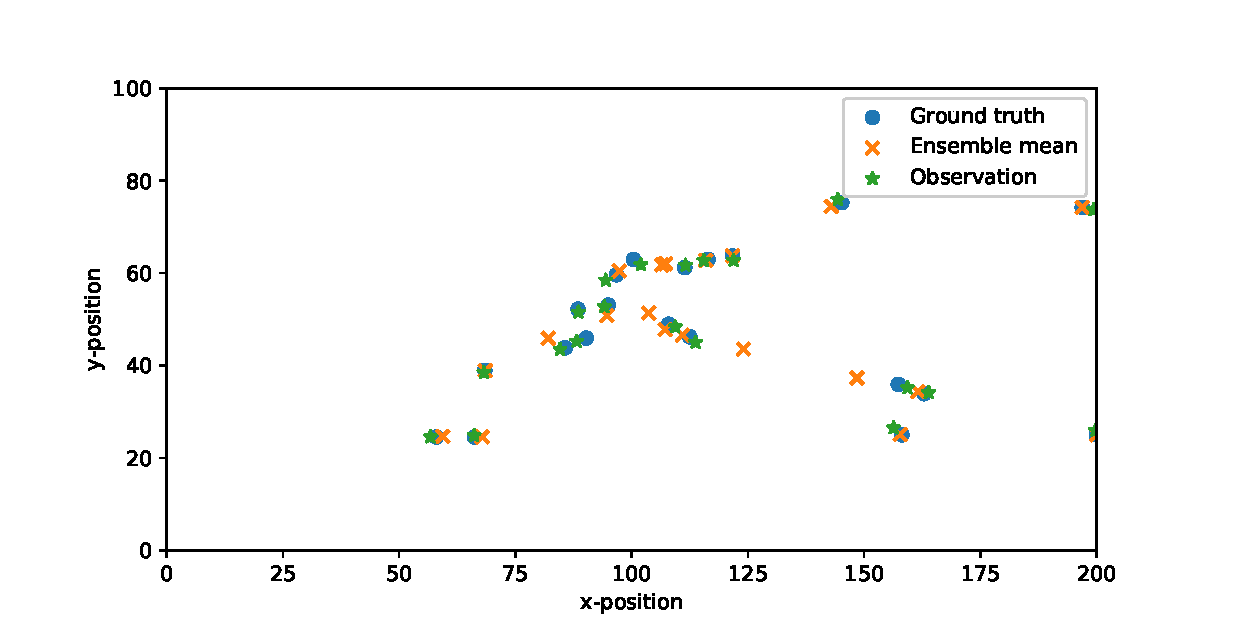
\includegraphics[width=\textwidth]{before_update_100.eps}
        \caption{Before update.}\label{fig:abm_before}
    \end{subfigure}

    \begin{subfigure}[h]{\textwidth}
        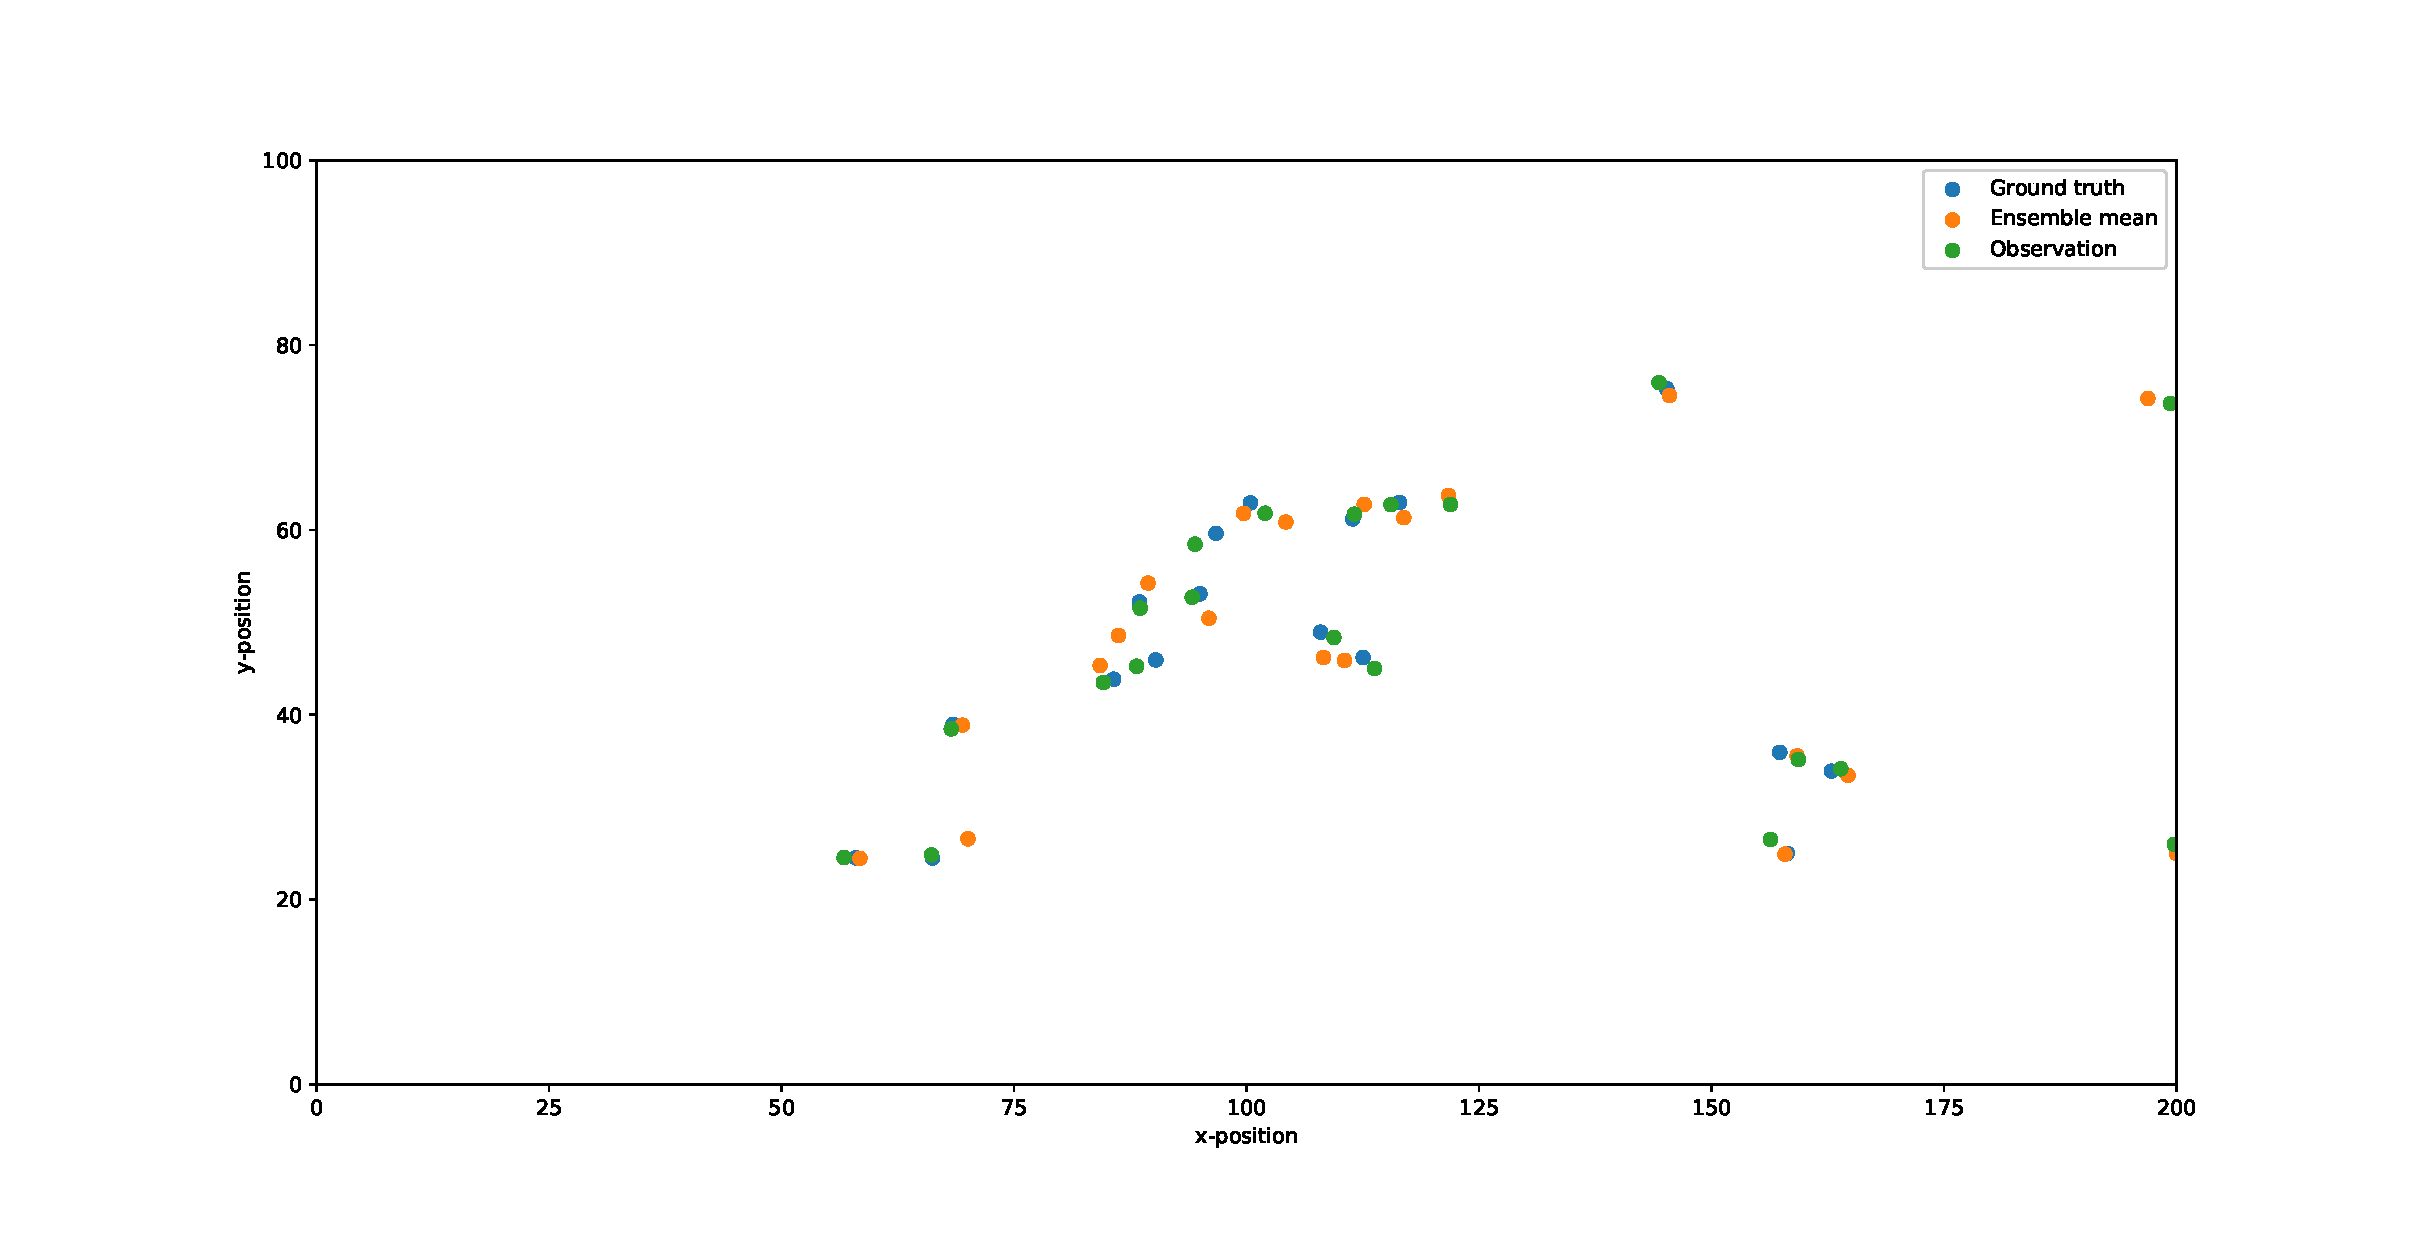
\includegraphics[width=\textwidth]{after_update_100.eps}
        \caption{After update.}\label{fig:abm_after}
    \end{subfigure}
    \caption[Effect of Ensemle Kalman Filter update on state of
    model.]{\centering Effect of Ensemble Kalman Filter update on state of model
    ($k=100$).}\label{fig:enkf_abm}
\end{figure}

It can be seen that in the case of many agents, the forecast position is already
very close to both the ground truth and the respect observation of the agent.
This is a consequence of the design of the model --- when unimpeded, agents take
as direct a route as possible towards their target destination.
As a result, in these cases, the agent motion simulated by \texttt{base\_model}
and by the filter ensemble members is often the same.
This can be observed in agents that have advanced ahead of others and are close
to reaching their respective exits, and in slower agents that lag behind (Figure
\ref{fig:abm_before}).
Where the ensemble mean agent position forecast is already close to the ground
truth, the application data assimilation has little effect, as revealed by
comparing Figures \ref{fig:abm_before} and \ref{fig:abm_after} for the
aforementioned selections of agents.

In cases where agents interact, however, we observe that the ground truth and
ensemble mean forecast differ; this can be seen where agents crowd near the
centre of the environment in Figure \ref{fig:enkf_abm} (e.g. agents whose
forecast positions lie in the range $80<x<125, 40<y<55$).
In the case of these agents, the forecast ensemble mean agent positions lie
further away from the ground truth; indeed the forecast for some agents may lie
closer to the ground truth for different agent than the ground truth of the
original agent. 
In these cases, it can be seen by comparing Figures \ref{fig:abm_before} and
\ref{fig:abm_after} that the application of the Ensemble Kalman Filter is
effective in updating the ensemble mean state such that the analysis position of
the agents is closer to the ground truth.

\section{Impact of Ensemble Kalman Filter on agent
state}\label{sec:results:agent}

Whilst the previous section sought to show the efficacy of the Ensemble Kalman
Filter in updating the model state to reduce the error with respect to the
ground truth, this section focuses in on the impact of the data assimilation
method on the state of one of the agents in the model.
In particular, this allows us to examine the effect of applying data
assimilation to the state of each of the ensemble members.

\begin{figure}[h!]
    \centering
    \begin{subfigure}[h]{\textwidth}
        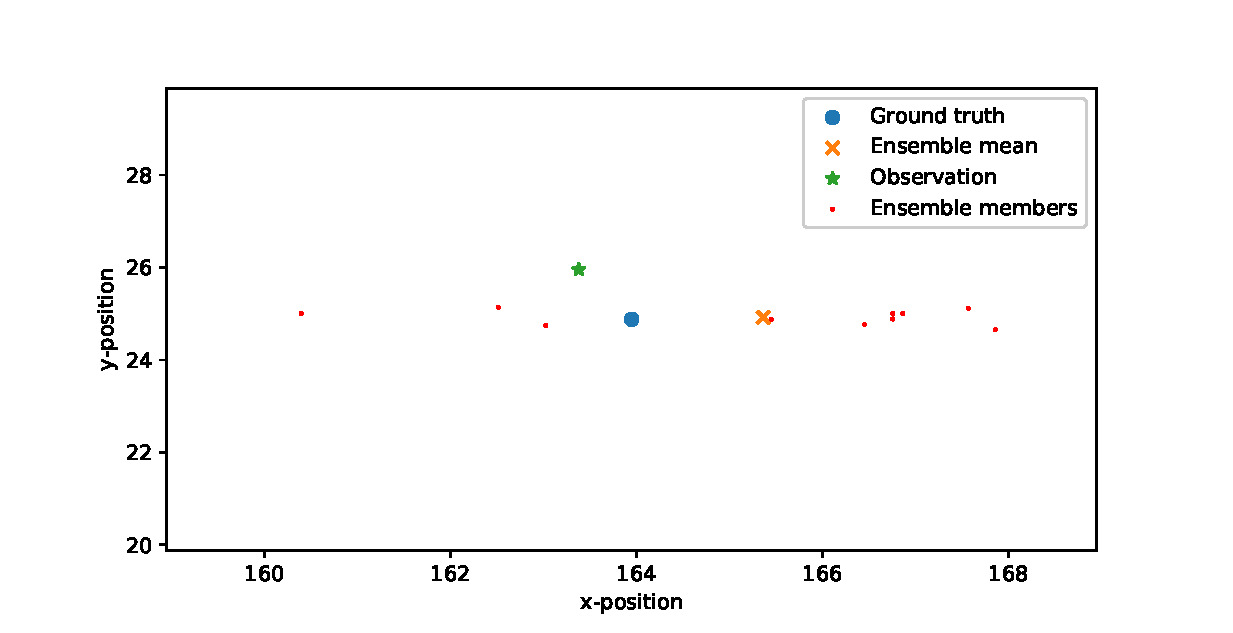
\includegraphics[width=\textwidth]{before_update_250_single.eps}
        \caption{Before update.}\label{fig:abm_before_single}
    \end{subfigure}

    \begin{subfigure}[h]{\textwidth}
        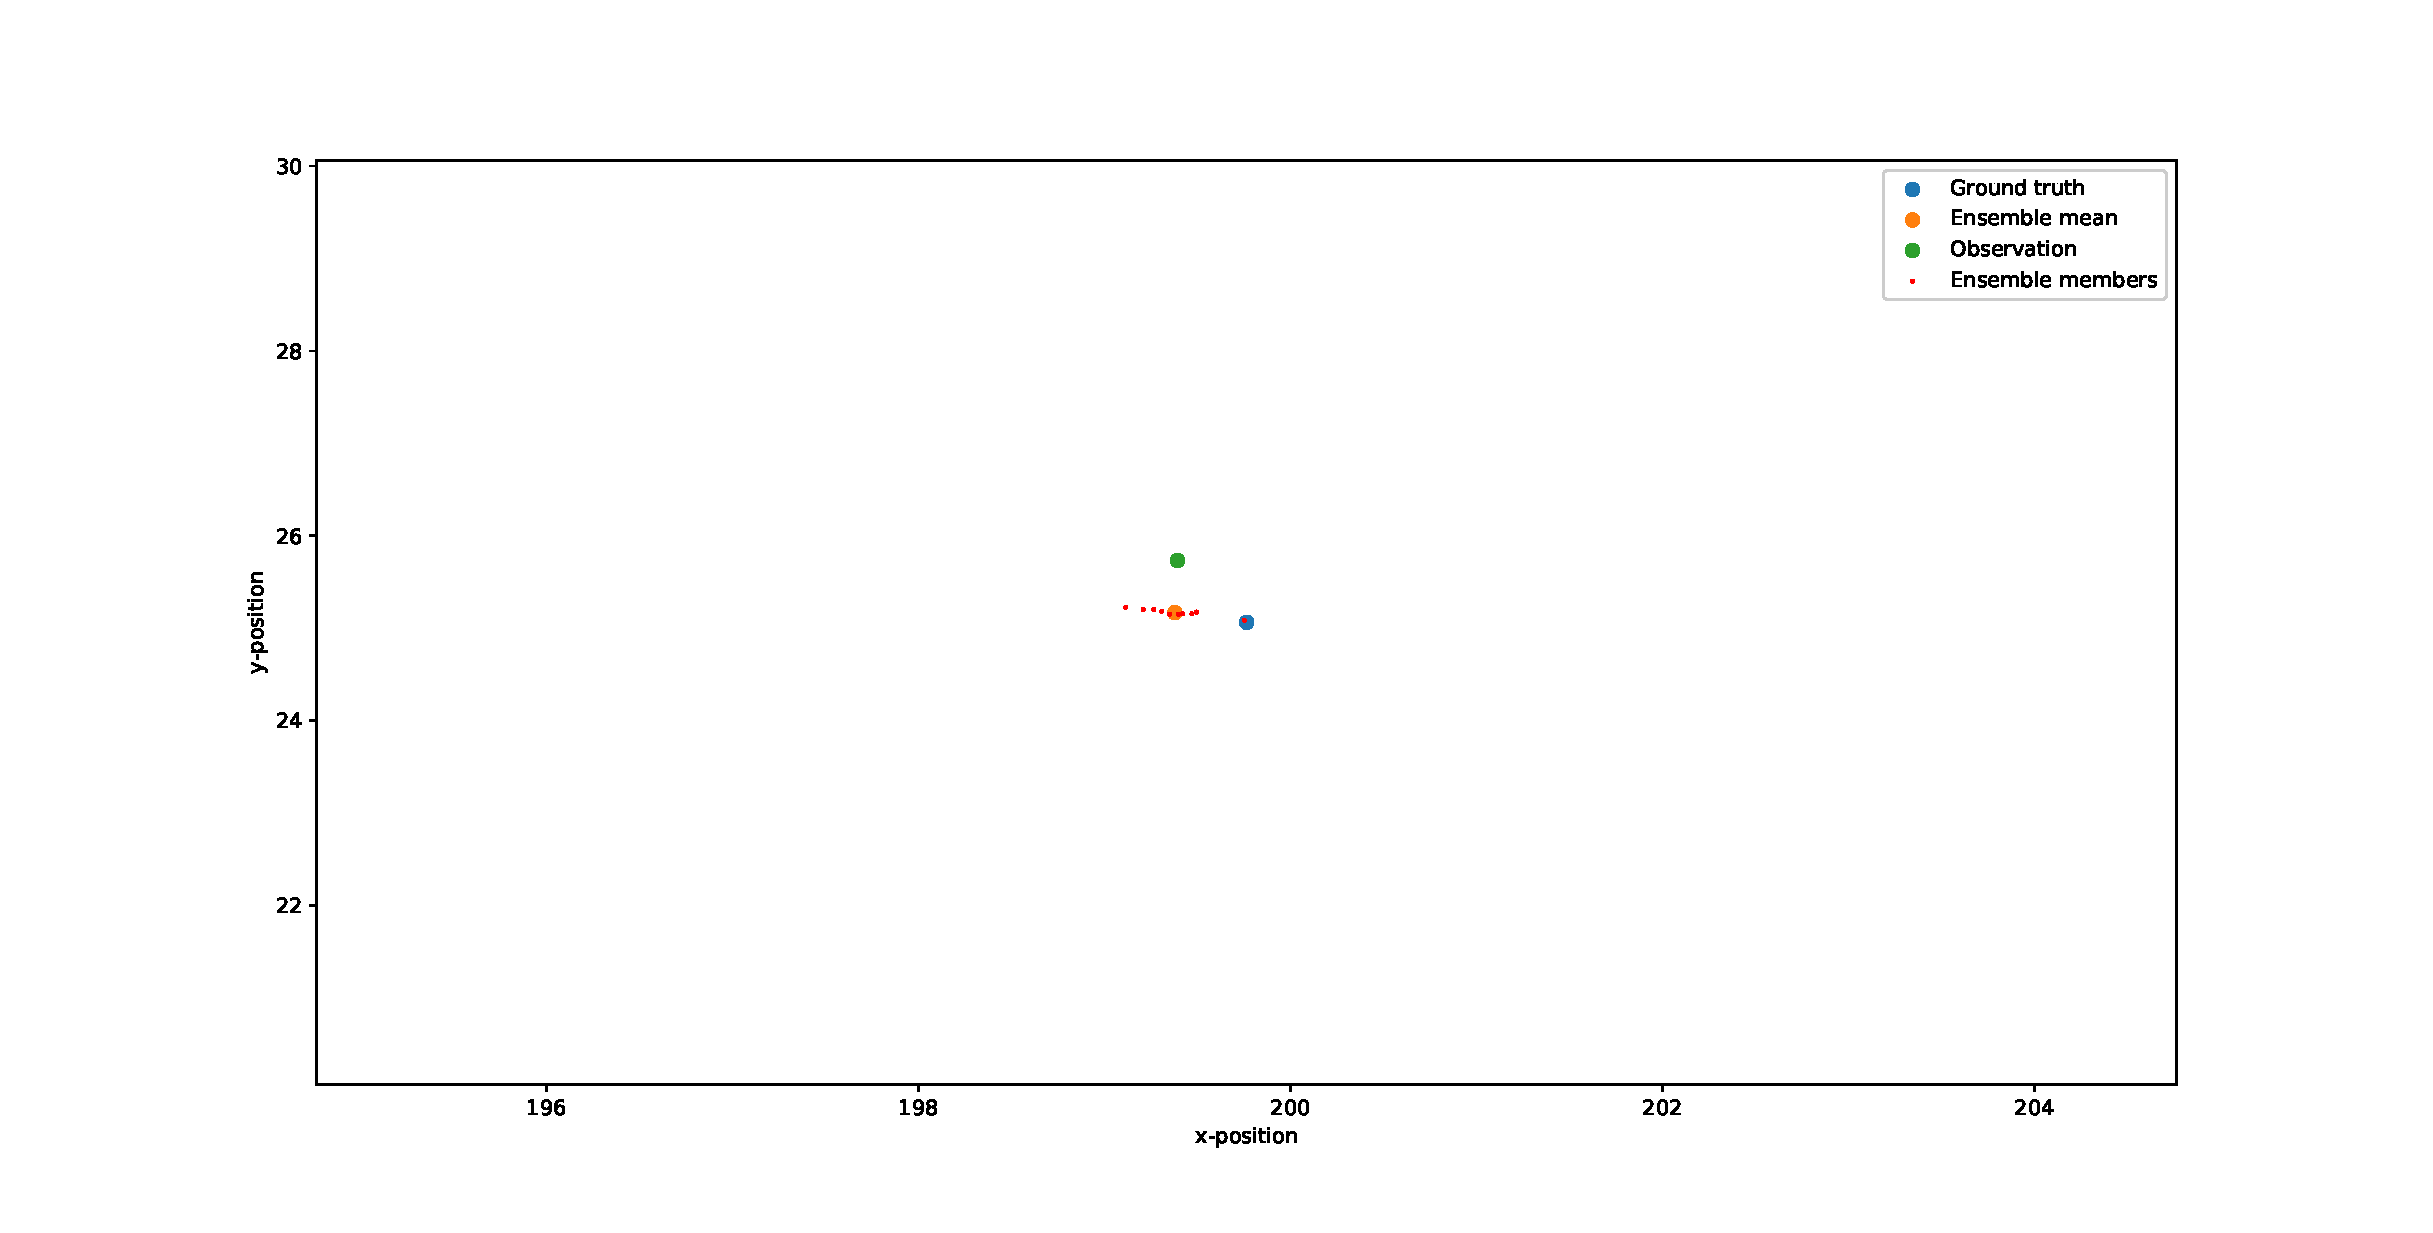
\includegraphics[width=\textwidth]{after_update_250_single.eps}
        \caption{After update.}\label{fig:abm_after_single}
    \end{subfigure}
    \caption[Effect of Ensemble Kalman Filter update on state of a single agent
    in the model.]{\centering Effect of Ensemble Kalman Filter update on state
    of a single agent in the model ($k=250$).}\label{fig:enkf_abm_single}
\end{figure}

In Figure \ref{fig:abm_before_single}, it can be seen that the error in the
forecast ensemble mean is only slightly worse than the observation error.
There is, however, large variation in the error of the members of the ensemble;
in the best case, one of the ensemble members exhibits error approximately equal
to the observation, but in the worst case, one of the ensemble members exhibits
error approximately four times that of the observation.
The forecast ensemble members appear to have diverged predominantly in the
$x$-direction, indicating that the dispersion is likely a result of the agent
getting stuck behind another in some of the ensemble realisations but not in
others.
Upon updating the model state based on the observation, the analysis ensemble
mean lies very close to the ground truth, greatly reducing the error in the
ensemble mean as seen in Figure \ref{fig:abm_after_single}.
The figure also shows that the error in the ensemble members falls as well, as
they converge on the ground truth.
This further confirms that the Ensemble Kalman Filter is effective in improving
the accuracy with which we can simulate pedestrian movement through agent-based
modelling.

\section{Comparison of errors in forecast, analysis and
observations}\label{sec:results:comparison}

Finally, we compare the error in the model forecasts, model analysis and
observations at each of the instances when data assimilation is undertaken (data
assimilation is undertaken every 50 time-steps).
The model forecast is taken to be the state produced by averaging the position
of each of the agents over the ensemble after undertaking the prediction
procedure, but before the update procedure; correspondingly, the model analysis
is taken to be the state produced by averaging the position of each of the
agents over the ensemble after having undertaken the update procedure.
The errors presented in Figure \ref{fig:rmse_comparison} are the root mean
squared error per agent at a given time-step $k$, where errors are taken in
euclidean distance between the true state and state given by the forecast,
analysis or observation:
\begin{equation}
    RMSE_{k}^{*} = \sqrt{\frac{1}{L} \sum_{j=0}^{L}
                    \left(
                    \| \mathbf{x}_{k}^{*} - \mathbf{x}_{k}^{t} \|_{2}
                    \right) ^ 2},
\end{equation}
where $L$ is the number of agents, $\mathbf{x}_{k}^t$ is the true agent position
at time-step $k$, $\mathbf{x}_{k}^{*}$ is the agent position for which we wish
to calculate the error at time-step $k$ (be it forecast position, analysis
position or observed position), and $\| * \|_2$ is the operator for calculating
the length of the contained vector known as the $2$-norm; for example,
$RMSE_{100}^{f}$ would represent the error in the forecast at $k=100$,
$RMSE_{200}^{a}$ would represent the error in the analysis at $k=200$, and
$RMSE_{300}^{o}$ would represent the error in the observations at $k=300$.
Figure \ref{fig:rmse_comparison} shows how the error for each of the forecast,
analysis and observation vary with each of the assimilation steps (for this
experiment, assimilation takes place every 50 time-steps).
The observations are produced by adding unbiased normally distributed random
noise with a standard deviation of $1$ to the true state, it is unsurprising to
observe that the error in the observations is consistently $1$ at each of the
assimilation steps.

\begin{figure}[h!]
    \centering
    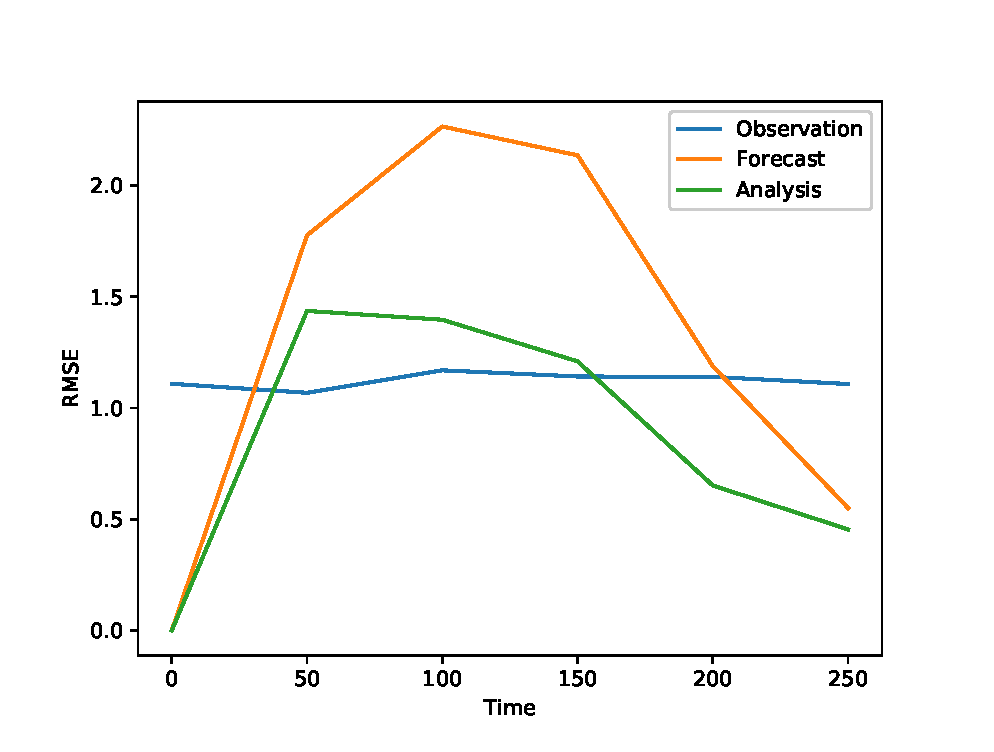
\includegraphics[width=\textwidth]{rmse_comparison.eps}
    \caption[Comparison of errors in model forecasts, model analysis and
    observations at each assimilation point.]{\centering Comparison of errors in
    model forecasts, model analysis and observations at each assimilation point;
    Root Mean Square Error (RMSE) is calculated relative to the ground truth
    with averaging performed over all agents.}\label{fig:rmse_comparison}
\end{figure}

Given that each of the realisations in the ensemble are initialised by taking a
deep-copy of the base-model used to produce truth data, both the forecast and
analysis errors at $k=0$ are $0$.
As model-time passes, the agents enter the model environment, interacting as
their paths cross.
These interactions inject some stochasticity into the model, and consequently
the error in the forecast grows; at $k=50$, we observe that $RMSE_{50}^{f}
\approx 1.75$.
The updating of the model state based on the observations at $k=50$ results in a
reduction in the model error to $RMSE_{50}^{a} \approx 1.4$ confirming, as in
Sections \ref{sec:results:model} and \ref{sec:results:agent}, that the data
assimilation scheme is effective in reducing model error.

The application of the Ensemble Kalman Filter at subsequent assimilation steps
continues to reduce the model error, with greater reductions being observed at
$k=100$ and $k=150$.
It is noteworthy that at $k=150$, where $RMSE_{150}^{f} > 2$ (i.e. over twice
the error in the observations), the observations perform only marginally better
than the analysis with $RMSE_{150}^{o} = 1.1$ and $RMSE_{150}^{a} = 1.2$.
Beyond this point in model-time, the model analysis outperforms the
observations, with $RMSE_{k}^{a} < RMSE_{k}^{o}$ for $k=200$ and $k=250$.

%\begin{figure}[h]
    %\centering
    %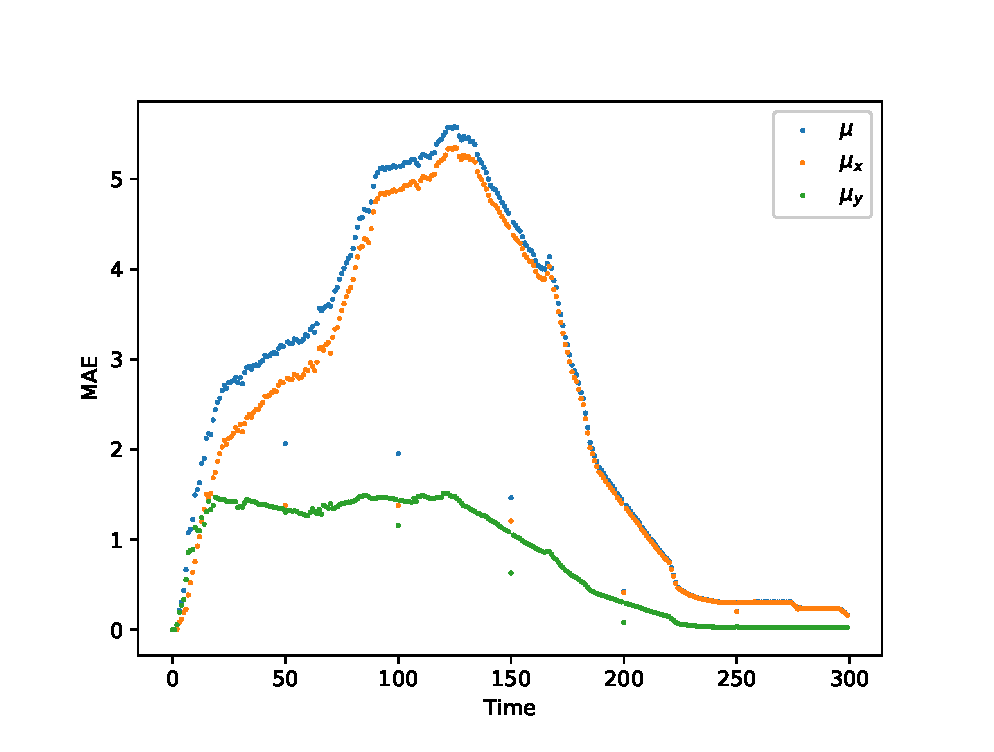
\includegraphics[width=0.8\textwidth]{errors}
    %\caption{Variation of errors with simulation time.}
    %\label{fig:errors}
%\end{figure}


\chapter{Conclusion}\label{ch:conclusion}

This is the conclusion.

\section{Future Work}\label{sec:conc:future}

Talk about the different types of EnKF and the implications for ensemble size
\citep{keller2018comparing}.
\begin{itemize}
    \item Damping: counteract filter divergence
    \item Localisation: reduce the effect of spurious correlations
    \item Hybrid EnKF: Covariance matrix is made up of the weighted sum of the
        usual covariance matrix and a separate static covariance matrix that
        encodes prior underlying knowledge about the system
    \item Dual EnKF: Split the state vector into state and parameters. At
        assimilation: update parameters, recalculate forecast, update state
    \item Normal Score EnKF: Developed to handle non-Gaussian PDFs in EnKF. At
        assimilation: transform state, parameters and measurements into
        Z-scores, perform EnKF update based on transformed values, transform
        back from Z-scores
    \item Iterative EnKF
\end{itemize}

Problems to consider:
\begin{itemize}
    \item What happens when agents leave the system --- does the filter
        recognise this correctly?
    \item What happens when we are provided with aggregated information?
    \item What happens when we are provided with different levels of information
        for different agents?
    \item Can the filter tell agents apart?
    \item We have artificially told the filter information about agents'
        entrance and exits - what happens if it doesn't know these? Do we then
        need to do some assimilation for data assimilation?
\end{itemize}

Ideas for transfer:
\begin{itemize}
    \item Explore impact of different filter parameters on filter performance
    \item Include derivation of multivariate Kalman filter
    \item Exploration of complexity of code (time and space)
    \item Multithreading to deal with computational cost - identifying cut-off
        point below which it is better to use serial computation. 
\end{itemize}

Extensions to the EnKF \cite{katzfuss2016understanding}:
\begin{itemize}
    \item Variance inflation: often have ensemble size much smaller than state
        dimension, which can mean that $\mathbf{K}$ can be a poor approximation
        of the kalman gain matrix; we can therefore get downwardly biased
        estimates of the posterior state covariance matrix ---  we can fix this
        with covariance inflation whereby we multiply the covariance matrix by a
        constant (greater than one).
    \item Localisation: small ensemble sizes can result in spurious
        correlations between state components that are physically far apart ---
        we can use localisation to avoid this.
    \item Parameter estimation: 
\end{itemize}


\begin{appendix}
    \appendix
\chapter{Code Documentation}\label{app:code_docs}

This is where I explain the design choices for how the enkf was coded.

\begin{itemize}
    \item options for generating observations:
        \begin{itemize}
            \item external
                \begin{itemize}
                    \item observations come from a previous model run as
                    synthetic data
                    \item therefore they should be independent
                    \item the problem here is that the ensemble members probably
                    have been set with the wrong entrances and exits or agents
                    \item this is likely more realistic, because when modelling
                    people we ultimately won't know where they intend to go
                    \item but we may be able to overcome this using parameter
                    estimation DA.
                \end{itemize}
            \item internal
                \begin{itemize}
                    \item observations come from the \texttt{base\_model}
                    \item all ensemble members are deep copies of the
                    \texttt{base\_model}
                    \item consequently, they have the same parameters and
                    initial conditions
                    \item problem here is that it's not very realistic
                    \item but we're going with it for this particular version
                \end{itemize}
        \end{itemize}
\end{itemize}


    \chapter{Bayes Rule}\label{ch:bayes_rule}

The joint probability --- $P(A, B)$ --- is the probability of event $A$ occurring
and event $B$ occurring.
The conditional probability --- $P(A | B)$ --- is the probability of event $A$
occurring given that event $B$ occurs.
The joint and conditional probabilities are linked by the following relationship:
\begin{equation}\label{eq:ab}
    P(A, B) = P(A) P(B | A).
\end{equation}
Similarly, we have
\begin{equation}\label{eq:ba}
    P(B, A) = P(B) P(A | B).
\end{equation}
Given that the joint probabilities of $A, B$ and $B, A$ are equal:
\begin{equation*}
    P(A, B) = P(B, A),
\end{equation*}
Equations \ref{eq:ab} and \ref{eq:ba} can be put together to give
\begin{equation}\label{eq:pre_bayes}
    P(A) P(B | A) = P(B) P(A | B).
\end{equation}
From this, we can derive the typical form of Bayes Rule by dividing by $P(A)$:
\begin{equation}\label{eq:bayes}
    P(B | A) = \frac{P(A | B) P(B)}{P(A)}.
\end{equation}

\end{appendix}

\bibliographystyle{agsm}
\bibliography{references}

\end{document}
